\subsubsection{逆映射的微商}

\begin{theorem}[Inverse Function Theorem]
    Let $D\subseteq\mathbb{R}^n$ be an open set, $F:\,D\to\mathbb{R}^n$ be a $C^1$ map. $F(x^0)=y^0$. Suppose $dF|_{x^0}:\,\mathbb{R}^n\to\mathbb{R}^n$ is invertible. i.e. $J_{x^0}(F)$ is invertible, then $\exists$ an open neighborhood $U$ of $x^0$, and an open neighborhood $V$ of $y^0$, s.t. $F|_U:\,U\to V$ is one-to-one, and the inverse $G:=(F|_U)^{-1}:\, V\to U$ is $C^1$, and $dG|_y=(dF|_{x=G(y)})^{-1}$\emph{, i.e. $J_yG=(J_xF)|_{x=G(y)}$}

    \begin{pf}
        Aim: For any $y$ near $y^0$, find $x$ s.t. $F(x)=y$\quad\raisebox{-0.5\height}{
\includegraphics[height=2cm]{chapters/09/03/0301}}

        Construct $H(x,y):\,\substack{D\times\mathbb{R}^n\to\mathbb{R}^n\\(x,y)\mapsto F(x)-y}$
        \begin{enumerate}
            \item $H\in C^1$
            \item $H(x^0,y^0)=F(x^0)-y^0=0$
            \item $(d_xH)|_{(x^0,y^0)}=dF|_{x^0}$ \emph{($J_xH=J_xF$, $J_yH=-Id$)} invertible
        \end{enumerate}

        $\overset{\text{Implicit Function Thm}}{\implies}\exists$ open neighborhood $V$ of $y^0$, and open neighborhood $\tilde{V}$ of $x^0$, s.t. $\{(x,y)\mid H(x,y)=0\}\cap(\tilde{V}\times V)=\{(G(y),y)\mid y\in V\}$ where $G:\,V\to\tilde{V}$ is the implicit function determined by $H=0$.

        $$G:\,V\to\tilde{V}\subseteq D$$

        Take $U\triangleq G(V)$, then\begin{align*}
            F|_U: & \,U\to V \\
            G:    & \,V\to U
        \end{align*}
        satisfies $\begin{cases}
                F|_U\circ G(y)=y & \forall y\in V \\
                G\circ F|_U(x)=x & \forall x\in U
            \end{cases}\rightarrow$ Since $F$ is continuous, $U$ is open. ($U=F^{-1}(V)\cap\tilde{V}$ open (since preimage of open set is open))

        \begin{center}
            
\includegraphics[height=5cm]{chapters/09/03/0302}
        \end{center}

        $F:\,\mathbb{R}^n\to\mathbb{R}^n$ continuous $\implies F^{-1}(\Omega)$ is open for any $\Omega$ open.

        \begin{center}
            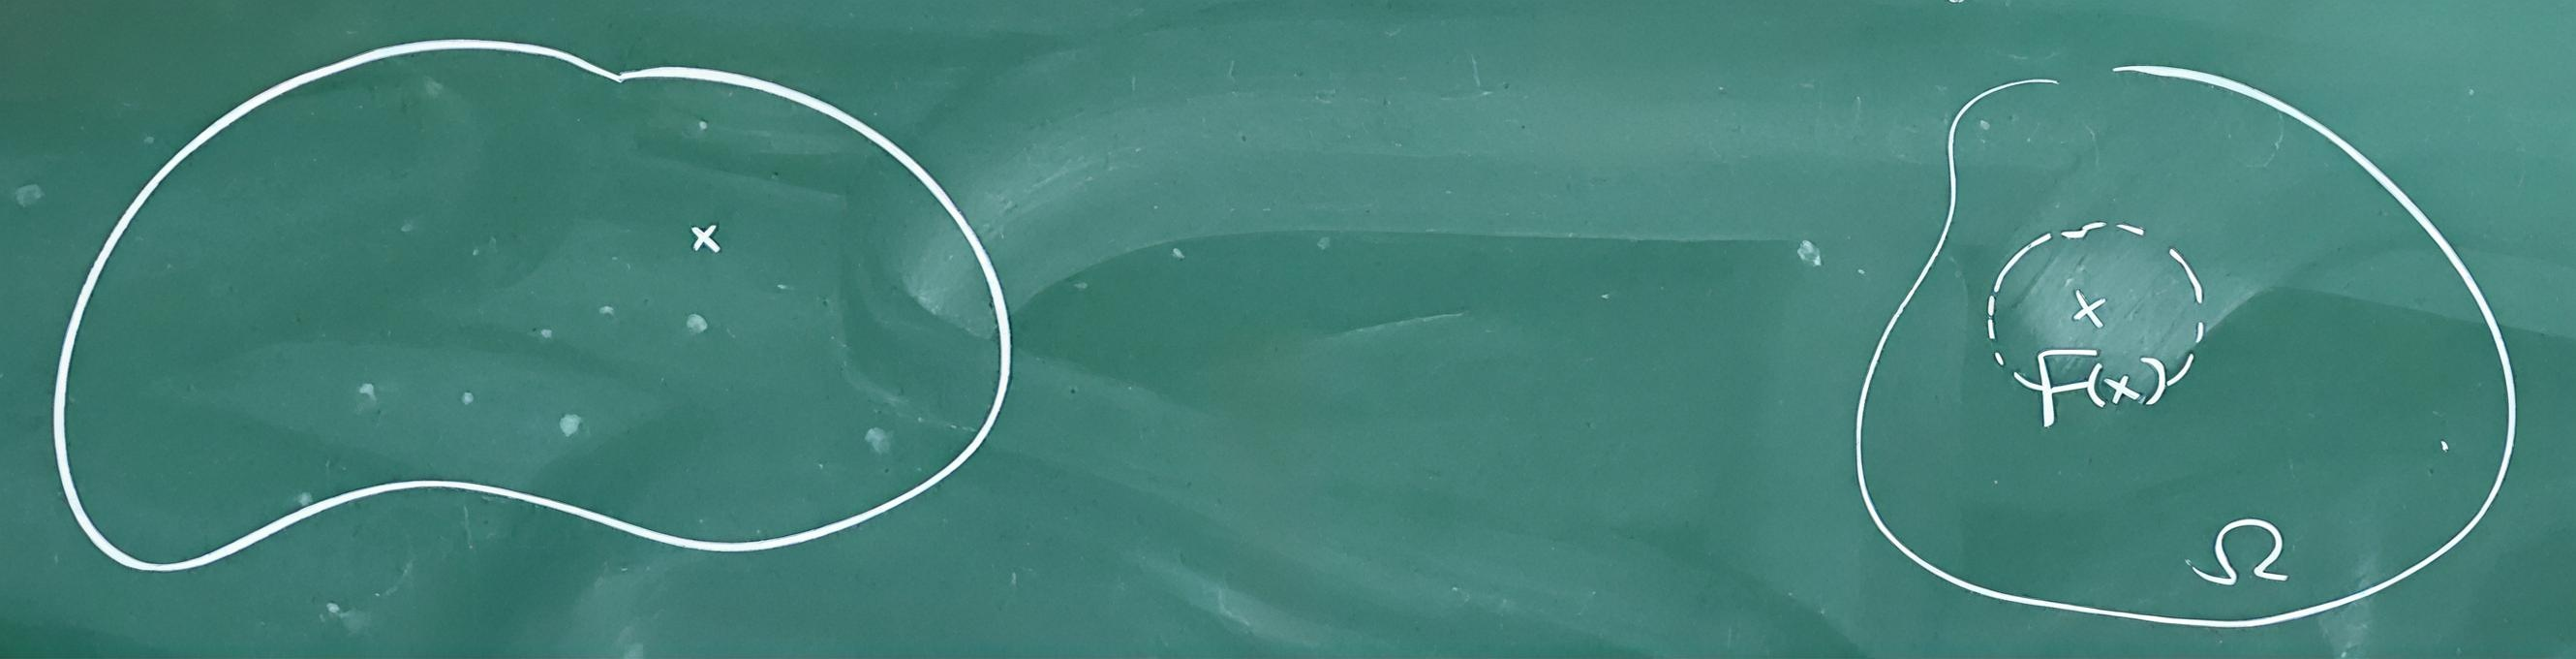
\includegraphics[height=3cm]{chapters/09/03/0303}
        \end{center}

        $\forall x\in F^{-1}(\Omega)$, i.e. $F(x)\in\Omega$, $\exists\varepsilon>0$ s.t. $B(F(x),\varepsilon)\subseteq\Omega$

        $\implies\exists\delta>0$ s.t. $F(B(x,\delta))\subseteq B(F(x),\varepsilon)\subseteq\Omega$

        $\implies B(x,\delta)\subseteq F^{-1}(\Omega)$

        Finally, differentiate, $F|_U\circ G(y)=y$, $y\in V$, we obtain $dF|_{x=G(y)}\circ dG|_y=id$

        $\implies dG|_y=(dF|_{x=G(y)})^{-1}$
    \end{pf}

    \paragraph*{Proof of Implicit Function Thm Using Inverse Function Thm}

    Aim: Sol $F(x,y)=0$ where $F:\,\mathbb{R}^n\times\mathbb{R}^m\to\mathbb{R}^m$

    Construct $H:,\substack{\mathbb{R}^n\times\mathbb{R}^m\to\mathbb{R}^n\times\mathbb{R}^m\\(x,y)\mapsto(x,F(x,y))}\leadsto J(H)=\left(\begin{array}{c|c}
                I_n  & 0    \\
                \hline
                J_xF & J_yF
            \end{array}\right)$

    Since $(J_yF)|_{(x^0,y^0)}$ invertible $\implies J_{(x^0,y^0)}(H)$ invertible $\overset{\text{Inverse Function Thm}}{\implies}\exists G=(H|_U)^{-1}:\,\underset{\text{neighborhood of }(x^0,0)}{V}\to\underset{\text{neighborhood of }(x^0,y^0)}{U}$ inverse

    $G(x,z)=(x,\varphi_z(x))$, then $\varphi_0(x)$ is the implicit function.

    $\substack{(x,\varphi_z(x))\mapsfrom(x,z)\\(x^0,y^0)\mapsto(x^0,0)}$\quad\raisebox{-0.5\height}{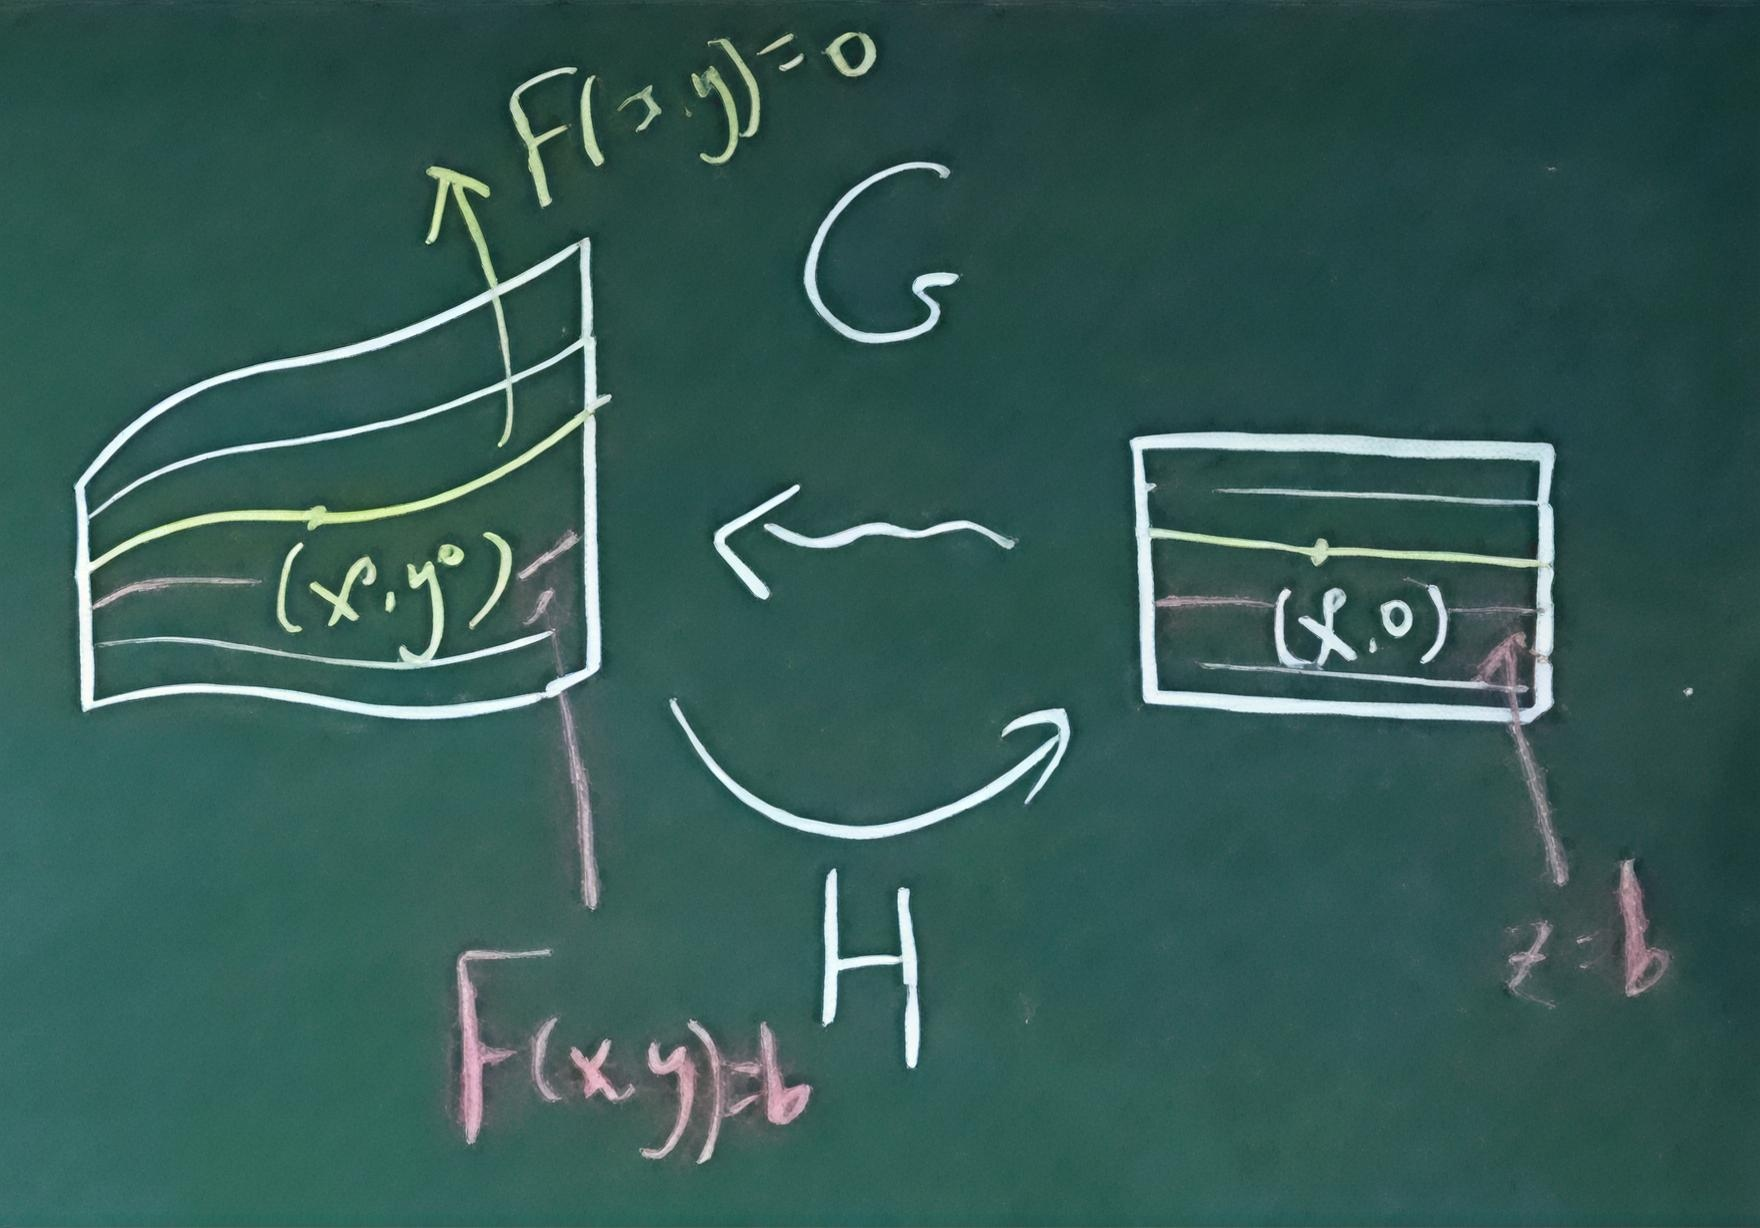
\includegraphics[height=2cm]{chapters/09/03/0304}}

    \begin{center}
        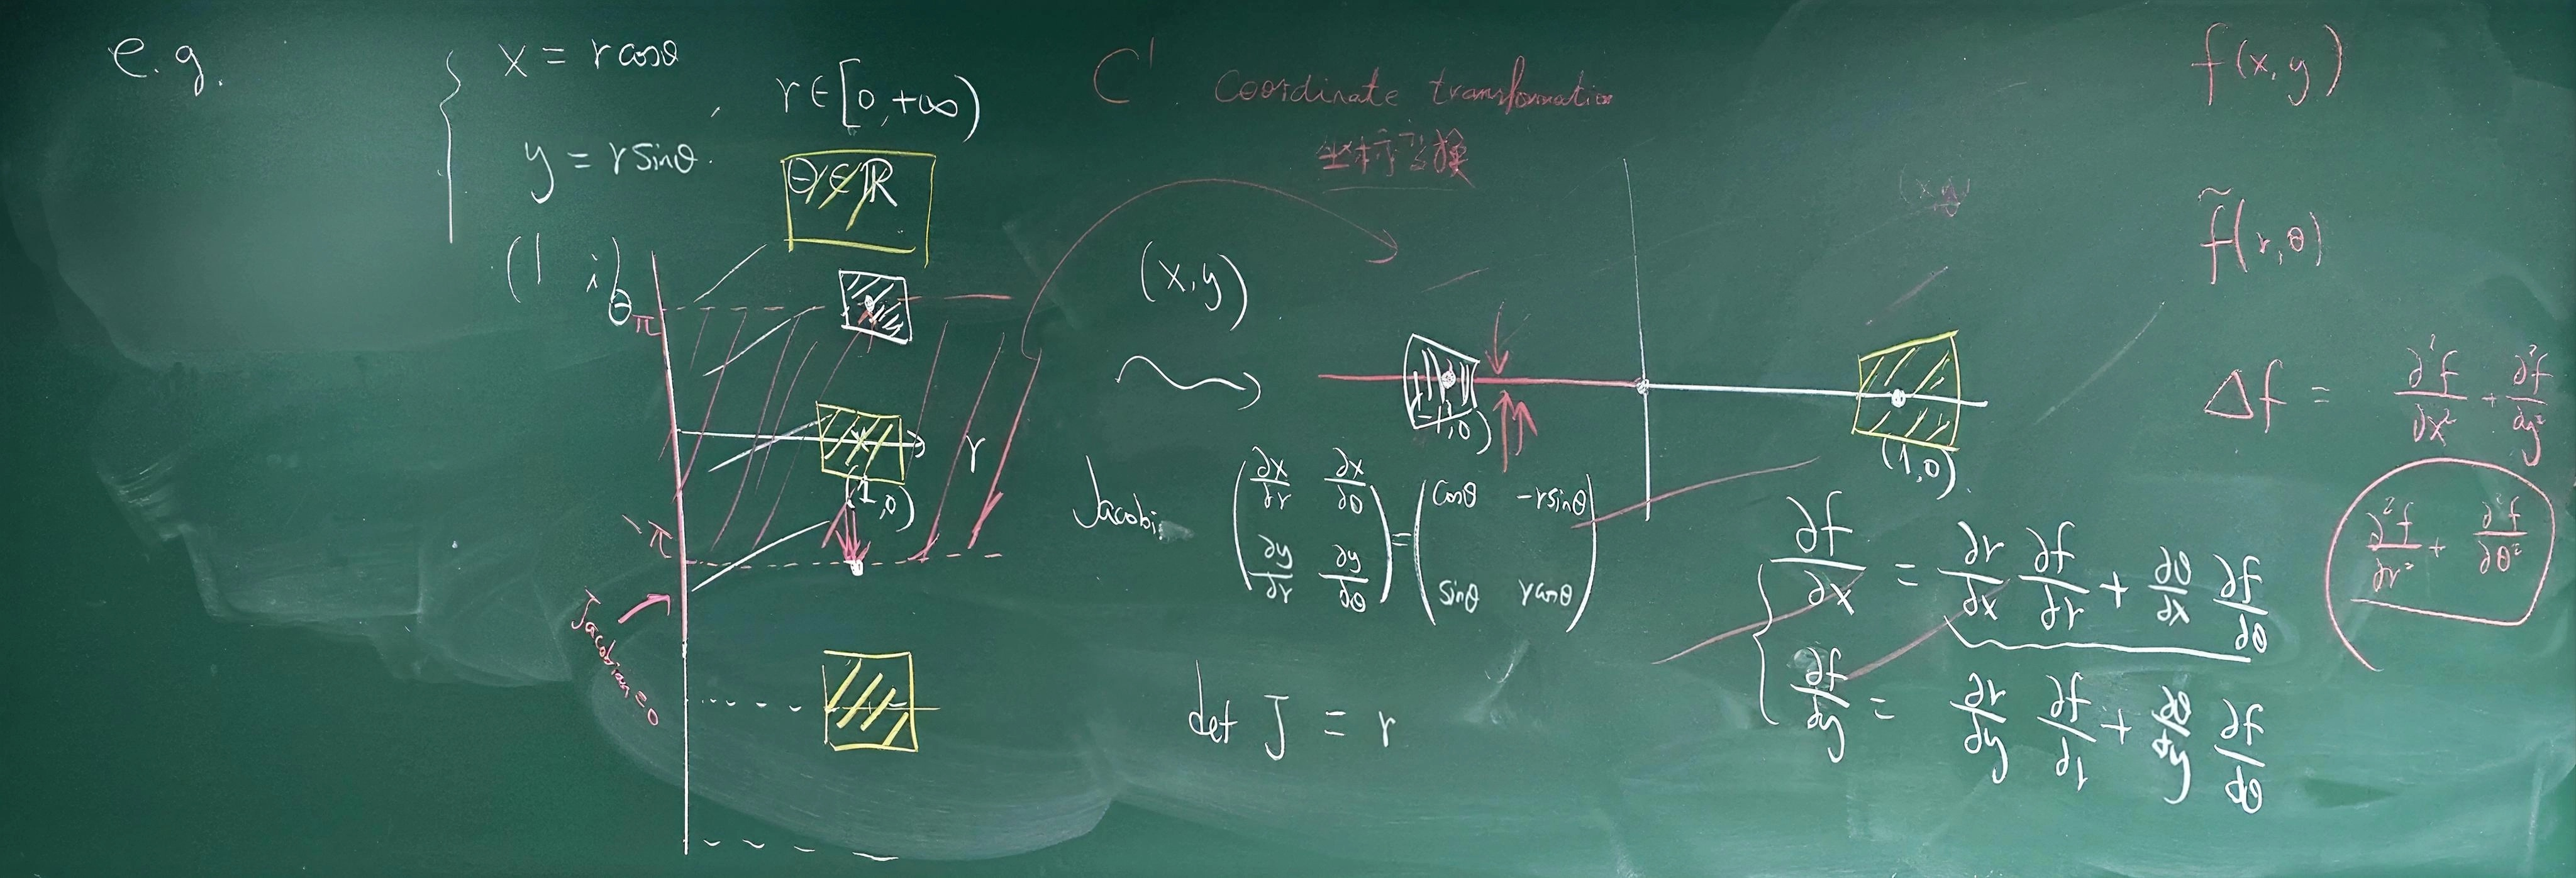
\includegraphics[width=\columnwidth]{chapters/09/03/0305}
    \end{center}

    $\begin{pmatrix}
            \frac{\partial f}{\partial x} \\
            \frac{\partial f}{\partial y}
        \end{pmatrix}
        =\begin{pmatrix}
            \frac{\partial r}{\partial x} & \frac{\partial\theta}{\partial x} \\
            \frac{\partial r}{\partial y} & \frac{\partial\theta}{\partial y}
        \end{pmatrix}
        \begin{pmatrix}
            \frac{\partial f}{\partial r} \\
            \frac{\partial f}{\partial\theta}
        \end{pmatrix}$

    $\frac{\partial}{\partial x}(\frac{\partial f}{\partial x})=\frac{\partial r}{\partial x}\frac{\partial}{\partial r}(\frac{\partial r}{\partial x}\frac{\partial f}{\partial r}+\frac{\partial\theta}{\partial x}\frac{\partial f}{\partial\theta})+\frac{\partial\theta}{\partial x}\frac{\partial}{\partial\theta}(\frac{\partial r}{\partial x}\frac{\partial f}{\partial r}+\frac{\partial\theta}{\partial x}\frac{\partial f}{\partial\theta})$

    $\Delta f=\frac{\partial^2f}{\partial r^2}+\frac{1}{r}\frac{\partial f}{\partial r}+\frac{1}{r^2}\frac{\partial^2f}{\partial\theta^2}$

    \begin{example}
        $\substack{f(x,y)=x\\\Delta f=0}\rightarrow\substack{\tilde{f}(r,\theta)=r\cos\theta\\\frac{1}{r}\cos\theta+\frac{1}{r^2}(-r\cos\theta)=0}$
    \end{example}

    $f(x,y,z)=r^{-1}$

    $f(x,y)=\log r=\log\sqrt{x^2+y^2}$

    $(\frac{1}{r})'+\frac{1}{r}\cdot\frac{1}{r}=0$
\end{theorem}



